% !TEX root = domain_transduction.tex
We evaluate our algorithm on various unsupervised domain adaptation tasks while focusing on two different problems, hand-written digit classification and object recognition.

%\subsection{Datasets and Baselines}
\vspace{2mm}
\noindent \textbf{Datasets:} We use MNIST~\cite{mnist}, Street View House Number~\cite{svhn} and the artificially generated version of MNIST -MNIST-M-~\cite{ganin15} to experiment our algorithm on the digit classification task. MNIST-M is simply a blend of the digit images of the original MNIST dataset and the color images of BSDS500~\cite{bsds500} following the method explained in \cite{ganin15}. Since the dataset is not distributed directly by the authors, we generated the dataset using the same procedure and further confirmed that the performance is the same as the one reported in \cite{ganin15}. Street View House Numbers is a collection of house numbers collected from Google street view images. Each of these three domains are quite different from each other and among many important differences, the most significant ones are MNIST being grayscale and the others being colored, and SVHN images having extra confusing digits around the centered digit of interest. Moreover, all domains are large-scale having at least 60k examples over 10 classes. 

In addition, we use the Office~\cite{office} dataset to evaluate our algorithm on the object recognition task. Office dataset includes images of the objects taken from Amazon, captured with a webcam and captured with a D-SLR. Differences between domains include the white background of Amazon images versus realistic webcam images, and the resolution differences. The Office dataset has fewer images, with a maximum of 2478 per domain over 31 classes. %On the other hand, it has larger number of classes over 31 categories.

%\subsection{Baselines}
\vspace{2mm}
\noindent \textbf{Baselines:} We compare our method with a variety of methods with and without feature learning. Considering the two different lines of work, \textbf{SA*}\cite{fernando13} is the dominant state-of-the-art approach not employing any feature learning, and \textbf{Backprop(BP)}\cite{ganin15} is the dominant state-of-the-art employing feature learning. We use the available source code of \cite{ganin15} and \cite{fernando13} and following the evaluation procedure in \cite{ganin15}, we choose the hyper-parameter of \cite{fernando13} as the highest performing one among various alternatives. We also compare our method with the \textbf{source only} baseline which is a convolutional neural network trained only using the source data. This classifier is clearly different from our nearest neighbor classifier; however, we experimentally validated that CNN always outperformed the nearest neighbor based classifier. Hence, we report the highest performing source only method.

\vspace{2mm}
\noindent \textbf{Evaluation:} We evaluate all algorithms in \emph{fully transductive} setup.  We feed training images and labels of the first domain as the source and training images of the second domain as the target. We evaluate the accuracy on the target domain as the ratio of correctly labeled images to all target images.



\subsection{Results}
Following the fully transductive evaluation, we summarize the results in Table~\ref{tab:res} and Table~\ref{tab:res2}. Table~\ref{tab:res} summarizes the results on the object recognition task using office dataset whereas  Table~\ref{tab:res2} summarizes the digit classification task on MNIST and SVHN.

\begin{table*}[ht]
\setlength{\tabcolsep}{3pt}
\caption{Accuracy of our method and the state-of-the-art algorithms on Office dataset.}
\vspace{-3mm}
\label{tab:res}
\begin{sc}
\begin{center}
\begin{small}
%\resizebox{\columnwidth}{!}{%
\begin{tabular}{@{}rcccccc@{}} \toprule 
 Source & Amazon & D-SLR & Webcam & Webcam &Amazon & D-SLR \\
 Target & Webcam & Webcam & D-SLR & Amazon & D-SLR & Amazon \\
 \midrule
GFK \cite{gong2012} & $.398$ & $.791$ & $.746 $ & $.371$ & $.379$ & .379   \\
SA* \cite{fernando13} & $.450$ & $.648$ & $.699$ & $.393$ & $.388$ & $.420$ \\
DLID \cite{chopra13} & $.519$ & $.782$ & $.899$ & -&- &- \\
DDC \cite{tzeng14} & $.618$ & $.950$ & $.985$ & $.522$ & $.644$& $.521$\\
DAN \cite{wang15} & $.685$ & $.960$ & $.990$ & $.531$ & $.670$ & $.540$ \\
Backprop \cite{ganin15} & $.730$ &$.964$ & $.992$ & $.536$ & $.728$ & $.544$\\
\midrule
Source Only & $.642$ & $.961$ & $.978$ & $.452$ & $.668$ & $.476$ \\
Our Method (k-NN only) & $.727$ &.952 & $.915$ & $.575$ & $.791$ & $.521$ \\
Our Method (no reject) & $.804$ &$.962$ & $.989$ & $.625$ & $.839$ & $.567$ \\
Our Method (full) & $\mathbf{.814}$ & $\mathbf{.971}$ & $\mathbf{.993}$ & $\mathbf{.663}$ & $\mathbf{.847}$ & $\mathbf{.601}$ \\
\bottomrule
\end{tabular}%}
\end{small}
\end{center}
\end{sc}
\vspace{-0mm}
\end{table*}

\begin{wraptable}{r}{0.5\textwidth}
\vspace{-2mm}
%\begin{table}[ht]
\setlength{\tabcolsep}{3pt}
\caption{Accuracy on the digit classification task.}
\vspace{-2mm}
\label{tab:res2}
\begin{sc}
\begin{small}
\resizebox{0.5\textwidth}{!}{%
\begin{tabular}{@{}r@{\hskip 1mm}c@{\hskip 1mm}c@{\hskip 1mm}c@{\hskip 1mm}c@{}} \toprule 
Source & M-M & MNIST  & SVHN & MNIST \\
Target&  MNIST & M-M & MNIST & SVHN\\
 \midrule
SA* \cite{fernando13}& $.523$ & $.569$ & $.593$ & $.211$ \\
BP \cite{ganin15} &$.732$ & $.766$ & $.738$ & $.289$ \\
\midrule
Source Only  & $.483$ & $.522$  &.549 & $.162$  \\
Our Method(k-NN only) & $.805$ & $.795$ & $.713$ & $.158$\\
Our Method(no reject) & $.835$ & $.855$ & $.774$ & $.323$\\
Our Method(full) & $\mathbf{.839}$ & $\mathbf{.875}$ & $\mathbf{.799}$ & $\mathbf{.413}$\\
 \bottomrule
\end{tabular}}
\end{small}
\end{sc}
\vspace{-2mm}
\end{wraptable}

Table~\ref{tab:res}\&\ref{tab:res2} shows results on object recognition and digit classification tasks covering all adaptation scenarios. Our experiments show that proposed method outperforms all state-of-the-art algorithms. Moreover, the increase in the accuracy is rather significant when there is a large domain difference such as \mbox{MNIST$\leftrightarrow$MNIST-M}, \mbox{MNIST$\leftrightarrow$SVHN}, Amazon$\leftrightarrow$Webcam and Amazon$\leftrightarrow$D-SLR. Our hypothesis is that the state-of-the-art algorithms such as \cite{ganin15} are seeking for features invariant to the domains whereas we seek for an explicit similarity metric explaining both differences and similarities of domains. In other words, instead of seeking for an invariance, we seek for an equivariance. %TODO(ozan): elaborate here



Table~\ref{tab:res2} further suggests our algorithm is the only one which can successfully perform adaptation from MNIST to SVHN. Clearly the features which are learned from MNIST cannot generalize to SVHN since the SVHN has concepts like color and occlusion which are not available in MNIST. Hence, our algorithm learns SVHN specific features by enforcing accurate transduction in the adaptation.

Another interesting conclusion is the asymmetric results. For example, the accuracy of adapting webcam to Amazon and adapting Amazon to webcam is significantly different. The similar behavior exists in MNIST and SVHN. This observation validates the importance of an asymmetric modeling.

To evaluate the importance of joint labelling and reject option, we compare our method with self baselines. Our self-baselines are versions of our algorithm not using reject option (\textbf{no reject}) and the version neither using reject option nor using joint labelling (\textbf{k-NN only}). Results on both experiments suggest that joint labelling and the reject option are both crucial for successful transduction. Moreover, reject option is more important when the domain shift is large (\eg MNIST$\rightarrow$SVHN). This is expected since transduction under large  shift is more likely to fail which can be prevented with reject option.

\begin{wrapfigure}{r}{0.4\textwidth}
\small
%\vspace{-5mm}
\begin{small}
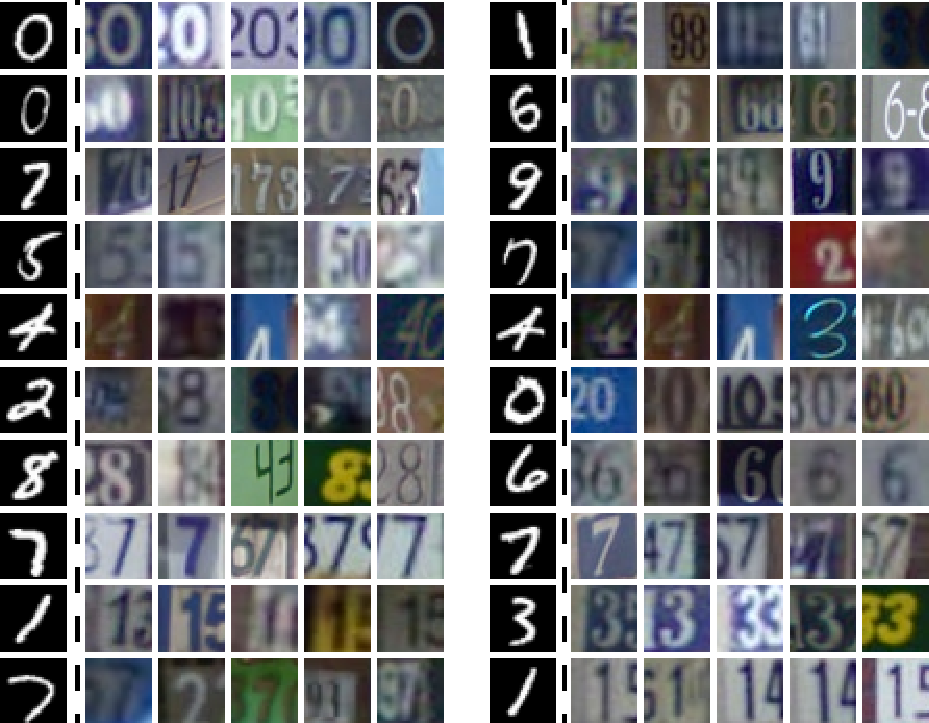
\includegraphics[width=0.4\textwidth]{nndig}
\vspace{-5mm}
\caption{Nearest neighbors for SVHN$\rightarrow$MNIST exp. We show an example MNIST image and its 5-NNs.}
\label{fig:nn}
%\end{figure}
%\begin{figure}[ht]
\includegraphics[width=0.4\textwidth]{nnfi-01.png}
\caption{Nearest neighbors for Amazon$\leftrightarrow$Webcam exp. We show an example Amazon image and its 3-NNs. }
%The drop in the accuracy after the nearest neighbors is expected since our loss function only models the nearest one.}
\label{fig:nnoffice}
\end{small}
\vspace{-5mm}
\end{wrapfigure}





\subsubsection{Qualitative Analysis}
To further study the learned representations and the similarity metric, we performed a series of qualitative analysis in the form of nearest neighbor and tSNE\cite{tsne} plots.


Figure~\ref{fig:nn} visualizes example target images from MNIST and their corresponding source images. First of all, our experimental analysis suggest that MNIST and SVHN are the two domains with the largest difference. Hence, we believe MNIST$\leftrightarrow$SVHN is very challenging set-up and despite the huge visual differences, our algorithm results in accurate nearest neighbors. On the other hand, Figure~\ref{fig:nnoffice} visualizes the example target images from webcam and their corresponding nearest source images from Amazon. 


The difference between invariance and equivariance is clearer in the tSNE plots of the Office dataset in Figure~\ref{fig:tsne} as well as digit classification task Figure~\ref{fig:tsnedigit}. In Figure~\ref{fig:tsne}, we plot the distribution of features before and after adaptation for source and target while color coding class labels. We use the learned embeddings as output of $\Phi_s$ and $\Phi_t$ as an input to tSNE algorithm\cite{tsne}. As Figure~\ref{fig:tsne} suggests, the source domain is well clustered according to the object classes with and without adaptation. Moreover, this is expected since the features are specifically fine-tuned to the source domain before the adaptation starts. However, target domain features have no structure before adaptation. This is also expected since the algorithm did not see any image from the target domain. After the adaptation, target images also get clustered according to the object classes. 




In Figure~\ref{fig:tsnedigit}, we show the digit images of source and target after the adaptation. In order to separately see the effect of common features and domain specific features, we compute the low-dimensional embeddings of the output of the shared network (output of the first fully connected layer). We further compute the NN points between source and target using $\Phi_s$ and $\Phi_t$, and draw an edge between NNs. Clearly, the target is well clustered according to the classes and source is not very well clustered although it has some structure. Since we learn the entire network for digit classification, our networks learn discriminative features in the target domain as our loss depends directly on classification scores in target domain. Moreover, discriminative features in target arises because of the transductive modeling. In comparison, state of the art domain invariance based algorithms only try to be invariant to the domains without explicit modeling of discriminative behavior on the target. Hence, our method explicitly models the relationship between the domains and results in an equivarient model while enforcing discriminative behavior in the target. 


%Another interesting observation is the unstable behavior when we disable label propagation. This is also expected since without label propagation, the labeling stage will have more mis-classifications and they will decrease the accuracy of the metric.
%>>>>>>> 495209cbd03d496cea6aa34df03ce5686deb5946


  
\begin{figure*}[ht]
    \begin{subfigure}[t]{0.25\textwidth}
        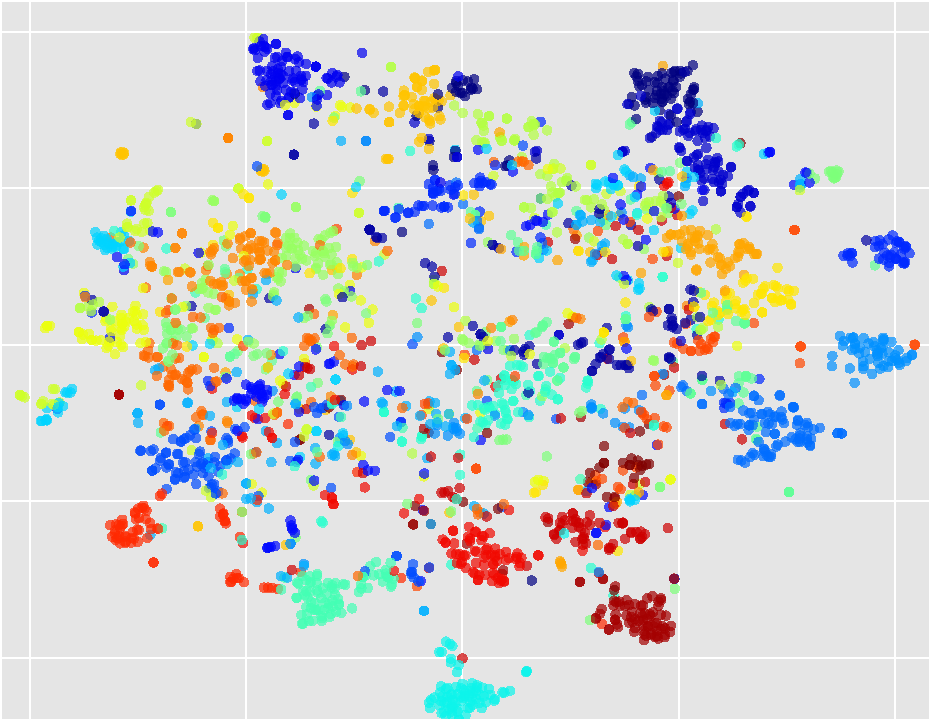
\includegraphics[width=\textwidth]{before_c_s_c}
        \caption{S. w/o Adaptation}
        \label{fig:gull}
    \end{subfigure}~\begin{subfigure}[t]{0.25\textwidth}
        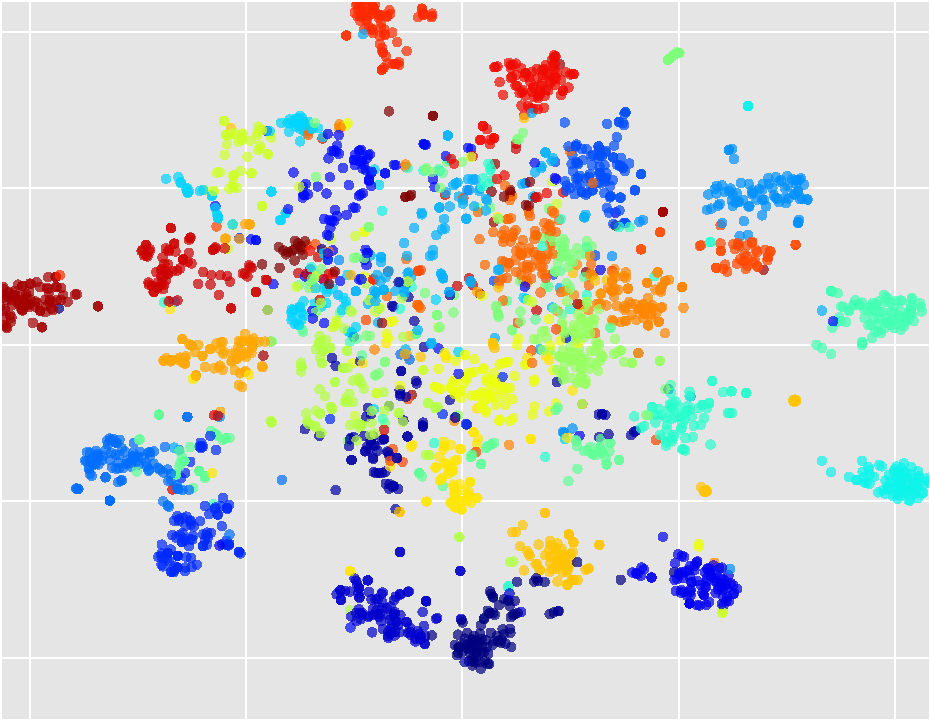
\includegraphics[width=\textwidth]{after_c_s_c}
        \caption{S. with Adaptation}
    \end{subfigure}~\begin{subfigure}[t]{0.25\textwidth}
        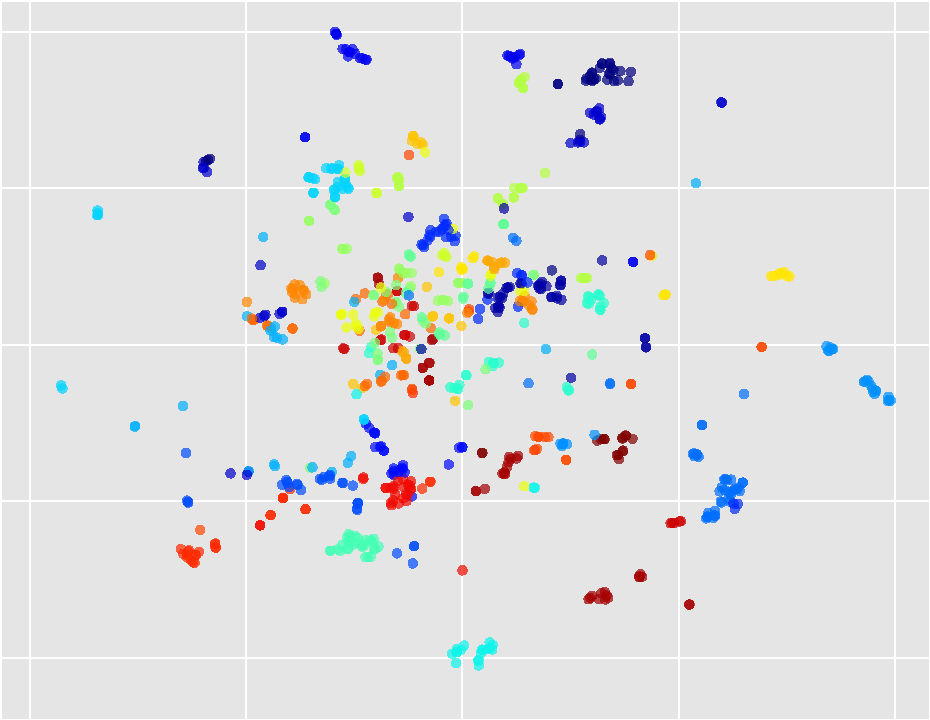
\includegraphics[width=\textwidth]{before_c_t_c}
        \caption{T w/o Adaptation}
        \label{fig:gull}
    \end{subfigure}~\begin{subfigure}[t]{0.25\textwidth}
        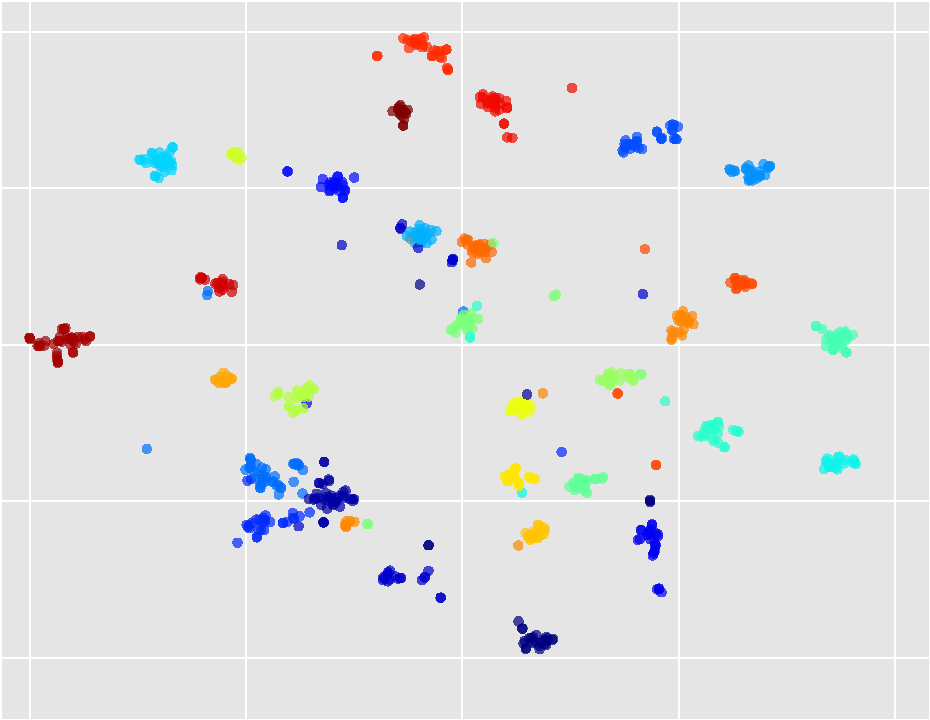
\includegraphics[width=\textwidth]{after_c_t_c}
        \caption{T with Adaptation}
    \end{subfigure}
    \caption{tSNE plots for office dataset Webcam(S)$\rightarrow$Amazon(T). Source features were discriminative and stayed discriminative as expected. On the other hand, target features became quite discriminative after the adaptation.}
    \label{fig:tsne}
        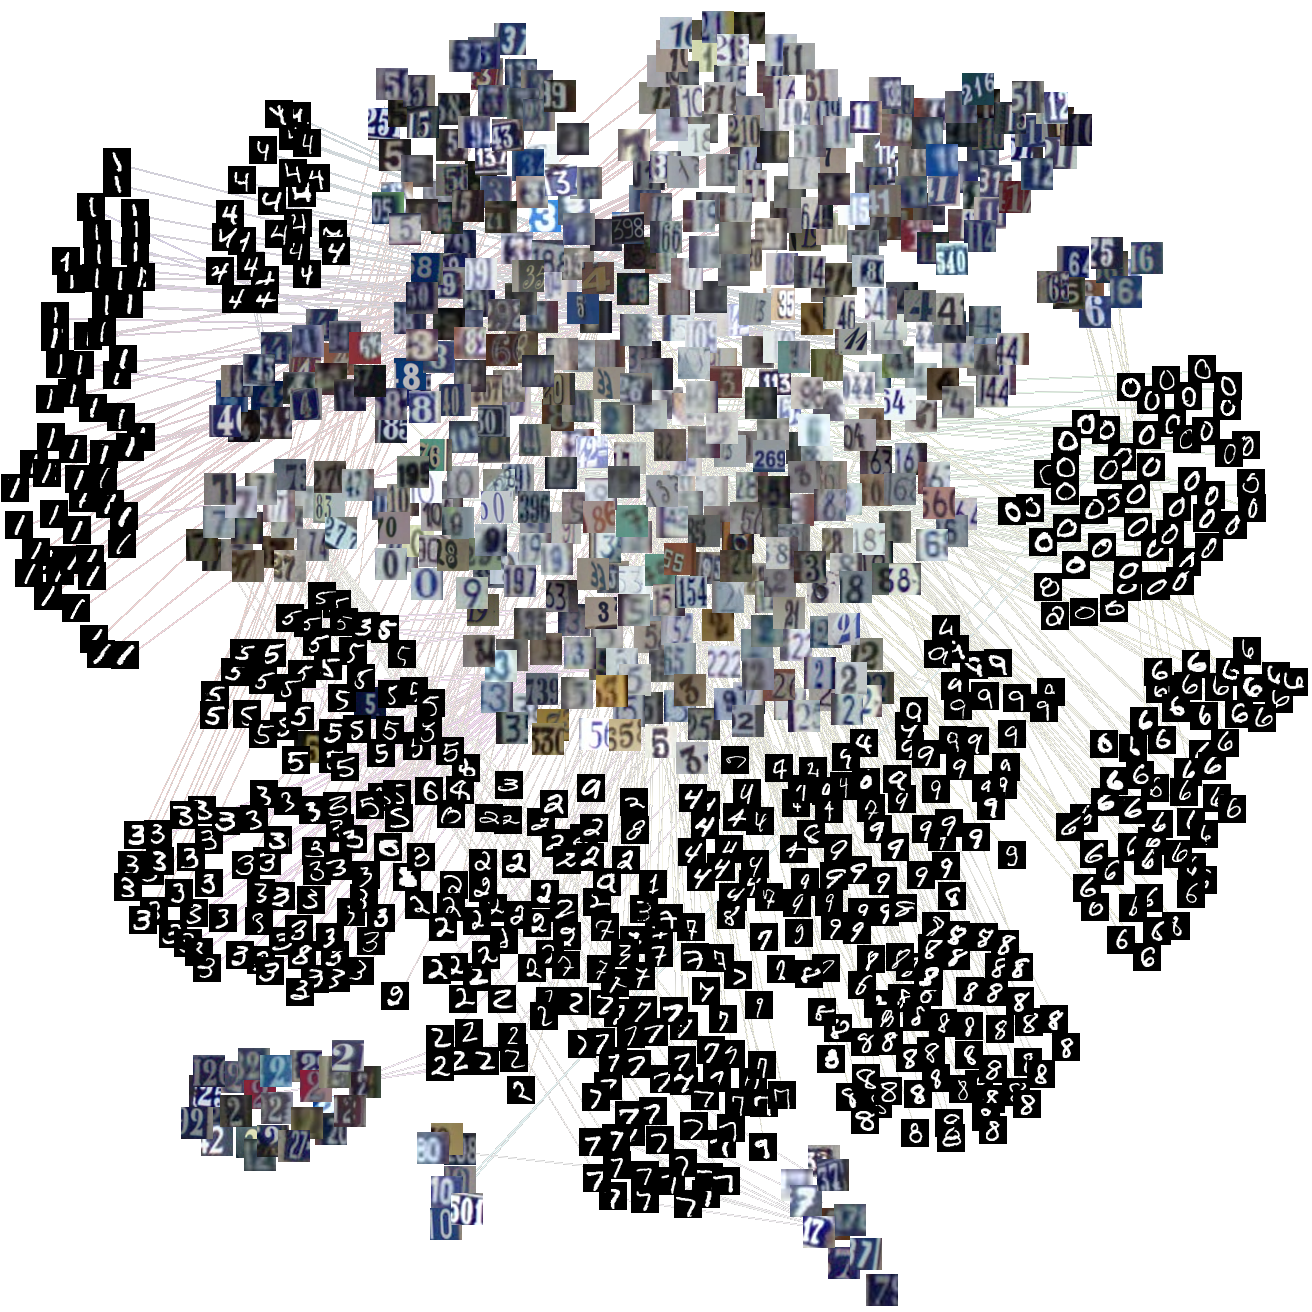
\includegraphics[width=\textwidth]{out_im.png}
        \vspace{-5mm}
\caption{tSNE plot for SVHN$\rightarrow$MNIST experiment. Please note that the discriminative behavior only emerges in the unsupervised target instead of the source domain. This explains the motivation behind modeling the problem as transduction. In other words, our algorithm is designed to be accurate and discriminative in the target domain which is the domain we are interested in.  }
\label{fig:tsnedigit}
\end{figure*}
